\section{Pendahuluan}
	Situs web merupakan suatu layanan yang menyajikan informasi menggunakan konsep hyperlink, yang memudahkan pengguna dalam menelusuri atau mencari informasi dari internet untuk mendapatkan informasi, dengan cukup mengklik suatu link beupa teks atau gambar, maka dari teks atau gambar tersebut akan menampilkan informasi yang detail (rinci).
Informasi yang akan disajikan dalam halaman web menggunakan konsep multimedia, informasi dapat disajikan dengan menggunakan banyak media (teks, gambar, animasi, suara (audio), dan film). Dalam suatu halaman web, informasi akan disajikan dalam kombinasi dari media-media tersebut yang disajikan dalam suatu halaman.

	Situs web berupa kumpulan informasi yang disediakan secara perorangan, kelompok, atau organisasi. yang ditempatkan setidaknya pada sebuah server web yang dapat diakses melalui jaringan seperti Internet, ataupun jaringan wilayah lokal (LAN) melalui alamat Internet yang dikenali sebagai URL. Gabungan atas semua situs yang dapat diakses publik di Internet disebut pula sebagai World Wide Web atau lebih dikenal dengan singkatan WWW. Web merupakan hal yang sangat populer di lingkungan pengguna internet dalam mengakses dan mendapatkan informasi karena kemudahan yang diberikan kepada pengguna internet untuk melakukan penelusuran, penjelajahan dan pencarian informasi. Dalam pembangungan web terbagi menjadi dua akan tetapi saling berkaitan yaitu: \textbf{Bahasa Pemrograman} dan \textbf{Web Server}.

\section{Bahasa Pemrograman}
PHP (Hypertext Preprocessor) adalah bahasa pemrograman script server-side yang didesain untuk pembuatan atau pengembangan web. Dengan ini, PHP juga dapat digunakan sebagai bahasa pemrograman umum. PHP sendiri dikembangkan pada tahun 1995
oleh Rasmus Lerdorf, dan pada akhhirnya dikelola oleh The PHP Group. Situs resmi PHP beralamat http://www.php.net.
PHP disebut bahasa pemrograman server side karena PHP diproses pada komputer server.  Hal ini berbeda dibandingkan dengan bahasa pemrograman client-side seperti JavaScript yang diproses pada web browser (client).
\par
Pada bulan Juni 1996, dirilis PHP/FI 2.0. Pada rilis ini interpreter PHP sudah diimplementasikan dalam program C. Dalam rilis ini disertakan juga modul-modul ekstensi yang meningkatkan kemampuan PHP/FI secara signifikan. Pada tahun 1997, sebuah perusahaan bernama Zend menulis ulang interpreter PHP menjadi lebih bersih, lebih baik, dan lebih cepat. Kemudian pada Juni 1998, perusahaan tersebut merilis interpreter baru untuk PHP dan meresmikan rilis tersebut sebagai PHP 3.0.
Pada pertengahan tahun 1999, Zend merilis interpreter PHP baru dan rilis tersebut dikenal dengan PHP 4.0. PHP 4.0 adalah versi PHP yang paling banyak dipakai pada awal abad ke-21. Versi ini banyak dipakai disebabkan kemampuannya untuk membangun aplikasi web kompleks tetapi tetap memiliki kecepatan dan stabilitas yang tinggi.
\par
Pada Juni 2004, Zend merilis PHP 5.0. Dalam versi ini, inti dari interpreter PHP mengalami perubahan besar. Versi ini juga memasukkan model pemrograman berorientasi objek ke dalam PHP untuk menjawab perkembangan bahasa pemrograman ke arah paradigma berorientasi objek. PHP juga banyak diaplikasikan untuk pembuatan program-program seperti sistem informasi  klinik, rumah sakit, akademik, keuangan, manajemen aset, manajemen bengkel dan lain-lain. Dapat dikatakan bahwa program aplikasi yang dulunya hanya dapat dikerjakan untuk desktop aplikasi, PHP sudah dapat mengerjakannya. Penerapan PHP saat ini juga banyak ditemukan pada proyek-proyek pemerintah seperti e-budgetting, e-procurement, e-goverment dan e e lainnya. Website Ubaya ini juga dibuat menggunakan PHP. PHP juga dapat dilihat sebagai pilihan lain dari ASP.NET/C /VB.NET Microsoft, ColdFusion Macromedia, JSP/Java Sun Microsystems, dan CGI/Perl. Contoh aplikasi lain yang lebih kompleks berupa CMS yang dibangun menggunakan PHP adalah Wordpress, Mambo, Joomla, Postnuke, Xaraya, dan lain-lain.

\subsection{Kelebihan PHP}
Dalam pembuatan program menggunakan PHP mempunyai kelebihan yaitu:
\begin{enumerate}
\item PHP dapat dijalankan diberbagai sistem operasi mulai Windows, Macintosh dan Linux.
\item PHP tidak perlu di compile
\item Mudah diinstall kedalam web server seperti apache sehingga konfigurasi menjadi mudah.
\item Pengembangan relatif mudah karena banyak yang membahas tentang PHP.
\end{enumerate}

\subsection{Penulisan Skript}
\begin{lstlisting}
Contoh:
<?php
 echo "Hello Word";
?>
\end{lstlisting}
PHP ini dapat dijalankan melalui file HTML yang kemudian akan dipanggil melalui web browser seperti Google Chrome, Mozilla Firefox dan UC Browser.
Program dalam PHP ditulis dengan ekstensi '.php'.

\subsection{PHP 7}
PHP 7 adalah rilis terbaru dari bahasa pemrograman PHP dan disebut sebagai revolusi dalam aplikasi web dapat dikembangkan dan dikirim untuk mobile. Rilis ini dianggap menjadi perubahan yang paling penting setelah perubahan dari PHP 5 pada tahun 2004. PHP7 dirancang untuk memiliki fitur bahasa pemograman yang lebih baik dari versi PHP yang sebelumnya dengan kecepatan yang mencapai 2 kali dari kecepatan PHP 5.6.x. PHP7 merupakan versi terbaru yang ditunggu oleh pengembang aplikasi web dengan menggunakan PHP, karena versi PHP sejak tahun 2004 berlabel versi 5 sebagai versi mayornya, dan juga sebagai versi yang terahir. versi 6 yang ditunggu kehadirannya terpaksa batal untuk dikeluarkan karena masalah teknis dalam perngembangannya.
Dalam PHP 7 terdapat beberapa fitur baru yaitu:
\begin{enumerate}
\item Improved Performance, memiliki kecepatan dua kali lebih cepat dari PHP 5.
\item Lower Memory Consumption, pemakaian memori yang rendah.
\item Consistent 64-bit support, dukungan konsisten untuk 64-bit mesin arsitektur.
\item Membuang konstruktor nama fungsi yang ada pada saat PHP4.
\item Operator baru yaitu spaceship dan interface.
\item Mengganti ekstensi JSON yang ada dengan JSOND.
\item Deklarasi tipe hasil dari suatu fungsi (return type).
\end {enumerate}

\section{Web Server}
Web server merupakan perangkat lunak yang menjadi bagian dari world wide web (www). Web server menunggu permintaan dari clinet dengan menggunakan sebuah browser seperti UC Browser, Google Chrome, Mozilla Firefox, dan browser lainnya. Jika ada permintaan melalui browser, maka web server akan memproses dan memberikan hasil proses kepada client. Web server ini bisa disebut sebagai perantara kita untuk mengolah web yang dibangun dan mengatur database. 

\begin{figure}[h]
\centering
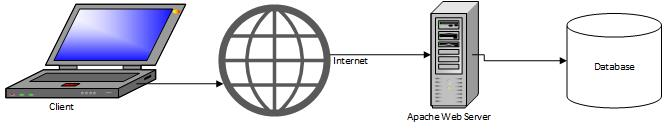
\includegraphics[scale=0.7]{figures/Alur-Web-Server}
\caption{Alur Web Server}
\label{webserver}
\end{figure}